\documentclass{article}

\usepackage{graphicx}
\graphicspath{ {images/} }
\usepackage{listings}
\lstset{inputpath=source}

%opening
\title{Quality Control Analysis based on Wait Times and Visit Lengths in Emergency Rooms Across the United States}
\date{\today}
\author{\textbf{Statistical Quality Control}\\
	Dr. Anthony Okafor\\
	University of West Florida\\
	\\ \\ \\ \\ \\ \\ \\ \\ \\
	Authors:\\
	Olga Akkan\\
	Derek Elliott\\
	Manuel Grossmann}

\begin{document}

\maketitle
\thispagestyle{empty}
\pagebreak
\cleardoublepage
\setcounter{page}{1}

\section*{Introduction}
Across the United States, ambulances are on average diverted away from an overcrowded emergency room approximately once every minute. Over the past decade, waiting times at emergency rooms have steadily increased, which often leads to frustration of the patients and their families. Long wait times will generally decrease patient satisfaction, and consequently the quality rating of an emergency room visit. Have you ever wondered how long the average person is waiting in the emergency room? The United States emergency department (ED) recommends an average wait of maximum 15 minutes. Leora Horwitz, Jeremy Green, and Elizabeth Bradley published an article called “United States emergency department performance on wait time and length of visit.” The following report will be based on their findings, where we will apply quality control processes to see if wait times in emergency rooms in within statistical control or if some adjustments may be necessary to improve the quality of a patients emergency room visit.
Horwitz, Green, and Bradley conducted a cross-sectional study of random sampling of 35,849 patient visits to 364 United States hospital emergency departments in 2006. They did not only measure the median wait times and visit lengths, but also the proportion of patients seen within the recommended time frame. The results are somewhat scary with conclusions that only a small minority of hospital consistently stayed within the suggested wait times. Additionally, they found that less than half of the hospitals ended up admitting their emergency room patients within 6 hours, meaning that many patients did in fact not necessarily need to visit the emergency room.

Methods
Horwith, Green, and Bradley examined the median ED performance with respect to the wait time, which they defined as the number of minutes between the patient arrived at the ED and the time the patient was seen by a provider. Secondly, the calculated the median length of the visit, defined as the number of minutes between the time the patient arrived at the ED and the time the patient was discharged from the ED. Both of these measures are directly correlated with customer satisfaction, and thus the quality of the emergency room visit. They categorized the wait times into four different triage categories:
\begin{itemize}
	\item Emergent(0-14 minutes)
	\item Urgent(15-60 minutes)
	\item Semi-urgent(61 minutes - 2 hours)
	\item Non-urgent(121 minutes - 24 hours)
\end{itemize}

For each of those categories, they calculated the percentage of patients seen within their triage target timeframe. They used standard descriptive statistics to characterize the sample of patients and hospitals. Additionally, they estimated linear models to identify the percent of variation in wait time (log-transformed) and in length of visit (log-transformed) within hospitals and between different hospitals. To perform such analysis, they used Stata 10.0 and SAS 9.1.2 depending on the analysis. The most important results are summarized in Table \ref{table:edwait}.
\begin{table}[]
	\centering
	\caption{Hospital performance on wait time and length of ED visit}
	\label{table:edwait}
	\begin{tabular}{|l|c|c|c|}
		\hline
		& Mean & Median & Proportion within target                                                        \\ \hline
		Wait time, all patients (min)                                                                     & 52.4 & 34.0   & 78.3\%                                                                          \\ \hline
		Emergent (min)                                                                                    & 31.8 & 16.0   & 48.4\%                                                                          \\ \hline
		Urgent (min)                                                                                      & 45.2 & 32.0   & 80.0\%                                                                          \\ \hline
		Semi-urgent (min)                                                                                 & 58.6 & 45.0   & 91.7\%                                                                          \\ \hline
		Non-Urgent (min)                                                                                  & 68.6 & 45.0   & 100\%                                                                           \\ \hline
		\begin{tabular}[c]{@{}l@{}}Length of visit,\\ patients ultimately admitted (hours)\end{tabular}   & 4.93 & 4.3    & \begin{tabular}[c]{@{}c@{}}76.3\% (6h target)\\ 60.0\% (4h target)\end{tabular} \\ \hline
		\begin{tabular}[c]{@{}l@{}}Length of visit,\\ patients ultimately discharged (hours)\end{tabular} & 3.0  & 2.3    & \begin{tabular}[c]{@{}c@{}}93.0\% (6h target)\\ 86.8\% (4h target)\end{tabular} \\ \hline
	\end{tabular}
\end{table}
As we can we from Table \ref{table:edwait}, most significant problem seems to be in the “emergent” triage category, where only 48.4\% of the patients are within the target of 0-14 minutes. This can possibly result in more damaging illnesses. This is where we will focus our attention to and use statistical quality control to assess if this process needs adjustments or not. http://www.ncbi.nlm.nih.gov/pmc/articles/PMC2830619/
\section*{Problem Statement}
The central tenet of quality improvement is that quality is a system property. ED wait time and length of visit have been observed to differ systematically according to race, ethnicity, site of care and a variety of other immutable patient-level factors. Using, instead, the quality improvement model, we examine ED wait time at the system (hospital) level. Describing hospital-level rather than patient-level performance allows for benchmarking, characterization of variation, recognition of positive and negative outliers, and assessment of effective care practices: activities necessary for sustainable quality improvement.
Let’s look at the data from https://projects.propublica.org/emergency/ which represents state-by-state waiting times for ERs. In Table \ref{table:stateave}, we chart the time, on average, that patients wait in emergency rooms before being seen by a doctor.
\begin{table}[]
	\centering
	\caption{Average ED wait time by State}
	\label{table:stateave}
	\begin{tabular}{|l|c|l|c|}
		\hline
		State         & \begin{tabular}[c]{@{}c@{}}Average Wait Time\\ (min)\end{tabular} & State          & \begin{tabular}[c]{@{}c@{}}Average Wait Time\\ (min)\end{tabular} \\ \hline
		Alabama       & 30                                                                & Montana        & 20                                                                \\ \hline
		Alaska        & 24                                                                & Nebraska       & 18                                                                \\ \hline
		Arizona       & 26                                                                & Nevada         & 21                                                                \\ \hline
		Arkansas      & 26                                                                & New Hampshire  & 28                                                                \\ \hline
		California    & 26                                                                & New Jersey     & 30                                                                \\ \hline
		Colorado      & 17                                                                & New Mexico     & 28                                                                \\ \hline
		Connecticut   & 27                                                                & New York       & 27                                                                \\ \hline
		Delaware      & 35                                                                & North Carolina & 30                                                                \\ \hline
		Florida       & 23                                                                & North Dakota   & 20                                                                \\ \hline
		Georgia       & 30                                                                & Ohio           & 20                                                                \\ \hline
		Hawaii        & 20                                                                & Oklahoma       & 23                                                                \\ \hline
		Idaho         & 20                                                                & Oregon         & 29                                                                \\ \hline
		Illinois      & 25                                                                & Pennsylvania   & 24                                                                \\ \hline
		Indiana       & 18                                                                & Rhode Island   & 31                                                                \\ \hline
		Iowa          & 20                                                                & South Carolina & 30                                                                \\ \hline
		Kansas        & 17                                                                & South Dakota   & 18                                                                \\ \hline
		Kentucky      & 22                                                                & Tennessee      & 23                                                                \\ \hline
		Louisiana     & 25                                                                & Texas          & 24                                                                \\ \hline
		Maine         & 27                                                                & Utah           & 16                                                                \\ \hline
		Maryland      & 46                                                                & Vermont        & 27                                                                \\ \hline
		Massachusetts & 35                                                                & Virginia       & 22                                                                \\ \hline
		Michigan      & 21                                                                & Washington     & 21                                                                \\ \hline
		Minnesota     & 25                                                                & West Virginia  & 27                                                                \\ \hline
		Mississippi   & 27                                                                & Wisconsin      & 18                                                                \\ \hline
		Missouri      & 23                                                                & Wyoming        & 17                                                                \\ \hline
		\multicolumn{3}{|l|}{National Average}                                                             & 24.54                                                             \\ \hline
	\end{tabular}
\end{table}
To improve productivity of ER we can construct and analyze Control Charts. 
Control charts have two general uses in an improvement project. The most common application is as a tool to monitor process stability and control. A less common, although some might argue more powerful, use of control charts is as an analysis tool.
Since natural subgroup size is unknown, we will construct The Individual (I) and Moving Range (MR) Charts for given data.
\pagebreak
\section*{Analysis}
The sample size of each of the measurements in Table \ref{table:stateave} is unknown, so the x-bar and R charts could not be used.  This made it a good candidate for an I and MR chart.  In Figure \ref{fig:ichart}, you can see the I chart for the data in Table \ref{table:stateave}.  As you can see from the figure, the Upper Control limit is 42.77, the Center Line is 24.54, and the Lower Control Limit is 6.31.  Only one data point fell outside of the control limits, and that corresponds to the state of Maryland.  This suggests that, except for Maryland, the states are within a three sigma range from the average national ED wait time.  The data in Table \ref{table:stateave} was collected between 2014 and 2015.  Previous data couldn't be found, which made the construction of an MR Chart impossible.  The chart in Figure \ref{fig:ichart} was generated in a custom script written in Python.  The code is included in Appendix I.
\begin{figure}
	\caption{I-Chart}
	\label{fig:ichart}
	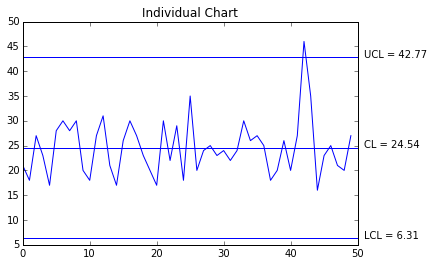
\includegraphics[width = \textwidth]{IChart}
\end{figure}

\pagebreak
\section*{Appendix I}
\lstinputlisting[language = Python]{qualiycontrol.py}



\end{document}